\chapter{Titration}\label{ch:g11:titration}

The box of an iron supplement promises \qty{80}{mg} of iron in every
tablet, as iron(II) \omterm{def:g9:ions:ion}{ions}. Is it true? A chemist crushes a tablet,
\omterm{def:g2:mixing-and-dissolving:dissolve}{dissolves} it in acid, and adds a purple solution of potassium
permanganate drop by drop from a long graduated tube. Each drop loses its
colour at once, as the permanganate \omterm{def:g9:ions:ion}{ions} are used up by the iron(II)
\omterm{def:g9:ions:ion}{ions}, until one drop, the last, leaves a faint pink that does not fade.
The volume poured at that moment gives the amount of iron. This chapter
turns a reaction into a measurement.

\begin{recall}
An \omterm{def:g11:redox:oxidant}{oxidant} gains \omterm{def:g9:inside-the-atom:nucleus}{electrons}, a \omterm{def:g11:redox:oxidant}{reductant} gives them; the permanganate \omterm{def:g9:ions:ion}{ion}
oxidises iron(II) \omterm{def:g9:ions:ion}{ions} according to
\ce{MnO4^- + 8H+ + 5Fe^{2+} -> Mn^{2+} + 5Fe^{3+} + 4H2O}
(\cref{ch:g11:redox}). \omterm{def:g10:concentration-and-dilution:molar-concentration}{Molar concentration} and \omterm{def:g10:concentration-and-dilution:dilution}{dilution}
(\cref{ch:g10:concentration-and-dilution}); the \omterm{def:g10:reaction-progress-table:extent}{progress table} and the
\omterm{def:g10:reaction-progress-table:limiting}{limiting reactant} (\cref{ch:g10:reaction-progress-table}).
\end{recall}

\begin{omfigure}
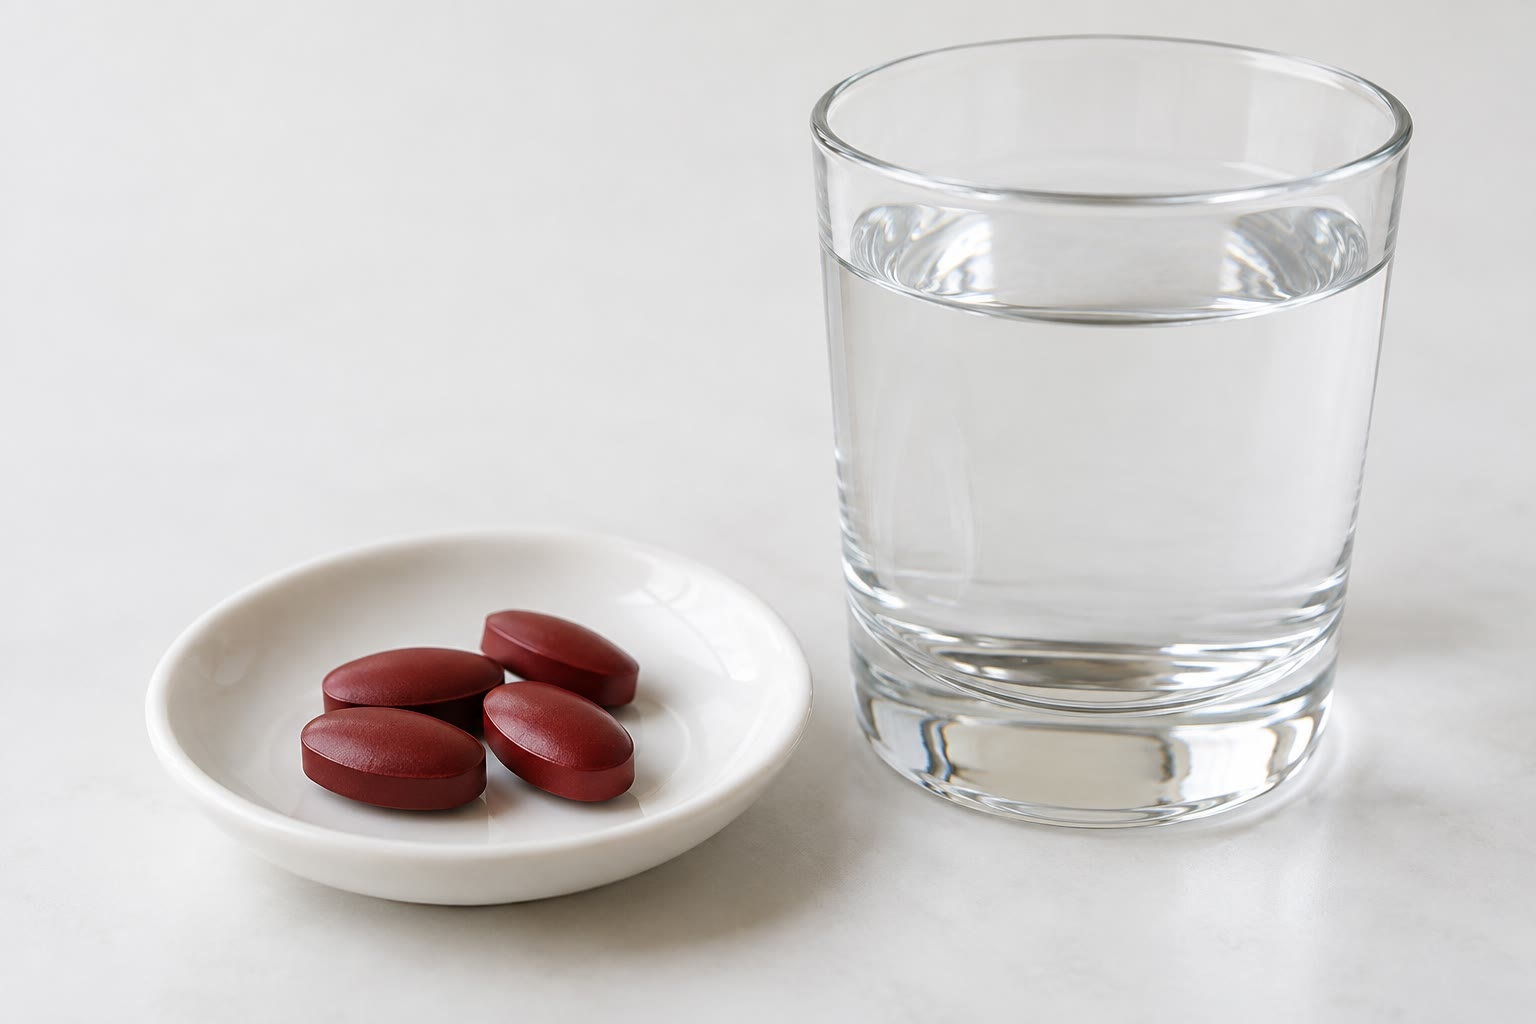
\includegraphics[width=0.45\linewidth]{images/book1/ai/g11-iron-tablets.jpg}

{\small Iron supplement tablets: how much iron does each really hold?}
\end{omfigure}

\section{Titrating}

\begin{definition}[Titration, titrant, titrated solution]\label{def:g11:titration:titration}
A \emph{titration}\index{titration} measures the amount of a dissolved
species by making it react with another species whose concentration is
accurately known. The solution of known concentration, added from a
burette, is the \emph{titrant}\index{titrant}; the solution containing
the species to be measured, placed in the flask, is the \emph{titrated
solution}\index{titrated solution}.
\end{definition}

\begin{proposition}[What a titration reaction must be]\label{prop:g11:titration:conditions}
A reaction can be used for a \omterm{def:g11:titration:titration}{titration} if it is total (so that one
\omterm{def:g7:chemical-reactions:reactant}{reactant} is entirely used up), fast (so that each drop reacts at once),
and unique (the \omterm{def:g11:titration:titration}{titrant} reacts with nothing else in the flask).
\end{proposition}

\begin{proof}
If the reaction stopped before completion, or lagged behind the drops,
or consumed \omterm{def:g11:titration:titration}{titrant} elsewhere, the volume poured would no longer measure
the amount of the titrated species.
\end{proof}

\begin{omfigure}
\begin{tikzpicture}[font=\small, scale=0.62]
  \pic[transform shape] at (0,0) {stand={5.8}{1.8}};
  \pic[transform shape] at (1.8,0.68) {stirrer};
  \pic[transform shape] at (1.8,0.68) {erlenmeyer={0.25}{yellow!12}};
  \pic[transform shape] at (1.8,2.98) {burette={0.75}{violet!55}};
  \draw[omProp, thick, <-] (2.15,6.9) -- (4.2,7.4) node[right, text=black,
    align=left] {burette: titrant\\ (potassium permanganate)};
  \draw[omProp, thick, <-] (2.55,1.4) -- (4.2,1.9) node[right, text=black,
    align=left] {conical flask: titrated\\ solution (iron(II), acid)};
  \draw[omProp, thick, <-] (3.0,0.4) -- (4.2,0.3) node[right, text=black]
    {magnetic stirrer};
\end{tikzpicture}

{\small A \omterm{def:g11:titration:titration}{titration} set: the burette, held on a stand, delivers the
\omterm{def:g11:titration:titration}{titrant} into the \omterm{def:g11:titration:titration}{titrated solution}, kept stirred.}
\end{omfigure}

\section{Equivalence}

\begin{definition}[Equivalence, equivalent volume]\label{def:g11:titration:equivalence}
\emph{Equivalence}\index{equivalence} is the moment of a \omterm{def:g11:titration:titration}{titration} when
the \omterm{def:g11:titration:titration}{titrant} added and the titrated species are in the proportions of the
equation: both are used up. The volume of \omterm{def:g11:titration:titration}{titrant} poured at that moment
is the \emph{equivalent volume}\index{equivalent volume}, $V_E$.
\end{definition}

\begin{proposition}[The relation at equivalence]\label{prop:g11:titration:relation}
For a \omterm{def:g11:titration:titration}{titration} reaction $a\,\ce{A} + b\,\ce{B} \longrightarrow$ products, with A titrated (amount
$n_A$) by a \omterm{def:g11:titration:titration}{titrant} B of concentration $c_B$, at \omterm{def:g11:titration:equivalence}{equivalence}
\[
  \frac{n_A}{a} = \frac{c_B\, V_E}{b} .
\]
\end{proposition}

\begin{proof}
At \omterm{def:g11:titration:equivalence}{equivalence} the \omterm{def:g6:pure-substances-and-mixtures:mixture}{mixture} is stoichiometric
(\cref{ch:g10:reaction-progress-table}): A and B, of initial amounts $n_A$
and $c_B V_E$, run out together, so $n_A / a = c_B V_E / b$.
\end{proof}

\begin{omfigure}
\begin{tikzpicture}
\begin{axis}[width=0.72\linewidth, height=5.6cm, xmin=0, xmax=20,
    ymin=0, ymax=16, xlabel={volume of titrant added (\si{mL})},
    ylabel={amount ($\num{e-4}$ \si{mol})}, axis lines*=left, ymajorgrids,
    grid style={gray!20}, tick label style={font=\small},
    label style={font=\small}, legend style={font=\small, at={(0.98,0.97)},
    anchor=north east, draw=none}, legend cell align=left]
  \addplot[very thick, orange!70!black, domain=0:14.3] {14.3 - x};
  \addplot[very thick, violet, domain=14.3:20] {0.2*(x - 14.3)};
  \addplot[very thick, violet, domain=0:14.3, forget plot] {0};
  \legend{\ce{Fe^{2+}} left in the flask, \ce{MnO4^-} in excess}
  \addplot[dashed, black!60] coordinates {(14.3,0) (14.3,7)};
  \node[font=\small, anchor=west] at (axis cs:14.5,6.5) {$V_E = \qty{14.3}{mL}$};
\end{axis}
\end{tikzpicture}

{\small Iron(II) titrated by permanganate at \qty{0.0200}{mol/L}: the
iron(II) \omterm{def:g9:ions:ion}{ions} run out exactly at the \omterm{def:g11:titration:equivalence}{equivalent volume}; after it, the
permanganate \omterm{def:g9:ions:ion}{ions} are no longer consumed and accumulate.}
\end{omfigure}

\section{Locating equivalence by a colour change}


\begin{proposition}[Seeing equivalence]\label{prop:g11:titration:colour}
When one of the species of the \omterm{def:g11:titration:titration}{titration} is coloured, \omterm{def:g11:titration:equivalence}{equivalence} is
seen as a colour change of the flask: the colour of the \omterm{def:g11:titration:titration}{titrant} appears
and persists as soon as the \omterm{def:g11:titration:titration}{titrant} is in excess, or the colour of the
titrated species disappears when it runs out.
\end{proposition}

\begin{proof}
Before \omterm{def:g11:titration:equivalence}{equivalence}, every \omterm{def:g9:ions:ion}{ion} of \omterm{def:g11:titration:titration}{titrant} that falls into the flask is
used up at once; after \omterm{def:g11:titration:equivalence}{equivalence}, it remains. A coloured species is
therefore present in the flask on one side of \omterm{def:g11:titration:equivalence}{equivalence} only.
\end{proof}

\begin{example}[Permanganate, its own indicator]\label{ex:g11:titration:permanganate}
The permanganate \omterm{def:g9:ions:ion}{ion} \ce{MnO4^-} is deep purple, and the manganese \omterm{def:g9:ions:ion}{ions}
\ce{Mn^{2+}} it gives are almost colourless; the iron \omterm{def:g9:ions:ion}{ions} give the
solution only a pale yellow tint. Before \omterm{def:g11:titration:equivalence}{equivalence}, each purple drop
is decolourised as it falls; the first drop that is not marks
\omterm{def:g11:titration:equivalence}{equivalence}: the flask turns pale pink and stays so.
\end{example}

\begin{omfigure}
\begin{tikzpicture}[font=\small]
  \pic at (0,0) {erlenmeyer={0.3}{yellow!14}};
  \pic at (3.2,0) {erlenmeyer={0.3}{magenta!10}};
  \pic at (6.4,0) {erlenmeyer={0.3}{violet!45}};
  \node[align=center, anchor=north] at (0,-0.15) {before equivalence:\\
    pale yellow, each drop\\ decolourised};
  \node[align=center, anchor=north] at (3.2,-0.15) {at equivalence:\\
    a faint pink that\\ persists};
  \node[align=center, anchor=north] at (6.4,-0.15) {after equivalence:\\
    purple (permanganate\\ in excess)};
\end{tikzpicture}

{\small The flask of an iron(II) \omterm{def:g11:titration:titration}{titration} by permanganate, before, at
and after \omterm{def:g11:titration:equivalence}{equivalence}. The \omterm{def:g11:titration:equivalence}{equivalent volume} is read at the first lasting
pink.}
\end{omfigure}

\begin{example}[Vitamin C and iodine]\label{ex:g11:titration:vitamin-c}
% ledger: aw:C, aw:H, aw:O
Vitamin C, ascorbic acid \ce{C6H8O6} ($M = \qty{176.0}{g/mol}$), is a
\omterm{def:g11:redox:oxidant}{reductant}; iodine \ce{I2} oxidises it:
\[
  \ce{C6H8O6 + I2 -> C6H6O6 + 2H+ + 2I-} .
\]
\qty{10.0}{mL} of orange juice, with a little starch, are titrated by an
iodine solution at \qty{5.00e-3}{mol/L}. Before \omterm{def:g11:titration:equivalence}{equivalence} the iodine is
used up; the first drop in excess turns the starch dark blue. If
$V_E = \qty{5.70}{mL}$, the juice held
$n = \num{5.00e-3} \times \num{5.70e-3} = \qty{2.85e-5}{mol}$ of vitamin
C, that is \qty{5.0}{mg} in \qty{10.0}{mL}: \qty{0.50}{g/L}.
\end{example}

\section{Computing an unknown concentration}

\begin{method}[Computing a concentration from a titration]\label{met:g11:titration:computing}
\begin{enumerate}
  \item Write the \omterm{def:g8:balanced-equations:equation}{balanced equation} of the \omterm{def:g11:titration:titration}{titration} reaction and read
        the coefficients $a$ (titrated species) and $b$ (\omterm{def:g11:titration:titration}{titrant}).
  \item Read $V_E$ on the burette, and compute the amount of \omterm{def:g11:titration:titration}{titrant}
        poured, $n_B = c_B V_E$.
  \item At \omterm{def:g11:titration:equivalence}{equivalence}, $n_A = \dfrac{a}{b}\, c_B V_E$.
  \item Divide by the volume titrated: $c_A = n_A / V_A$. If the sample
        was diluted before \omterm{def:g11:titration:titration}{titration}, multiply by the \omterm{def:g10:concentration-and-dilution:dilution}{dilution factor}.
\end{enumerate}
\end{method}

\begin{example}[An iron(II) solution]\label{ex:g11:titration:iron}
\qty{20.0}{mL} of an iron(II) solution, acidified, need
$V_E = \qty{12.6}{mL}$ of permanganate at \qty{0.0200}{mol/L}. Here
$a = 5$ (\ce{Fe^{2+}}) and $b = 1$ (\ce{MnO4^-}):
$n(\ce{MnO4^-}) = 0.0200 \times 0.0126 = \qty{2.52e-4}{mol}$, so
$n(\ce{Fe^{2+}}) = 5 \times \num{2.52e-4} = \qty{1.26e-3}{mol}$, and
$c(\ce{Fe^{2+}}) = \num{1.26e-3} / 0.0200 = \qty{0.0630}{mol/L}$.
\end{example}

\section{The titration as a measurement}

\begin{inthelab}[Reading a burette]
The burette is rinsed with the \omterm{def:g11:titration:titration}{titrant}, filled, and its tip freed of \omterm{def:g4:air-a-mixture-of-gases:air}{air}
bubbles. The level is read at the bottom of the meniscus, with the eye
at the same height, before and after the \omterm{def:g11:titration:titration}{titration}: the volume poured is
the difference. Graduations are every \qty{0.1}{mL}, and a reading can be
estimated to \qty{0.05}{mL}. Near \omterm{def:g11:titration:equivalence}{equivalence} the \omterm{def:g11:titration:titration}{titrant} is added drop
by drop, while the flask is swirled or stirred.
\end{inthelab}

\begin{omfigure}
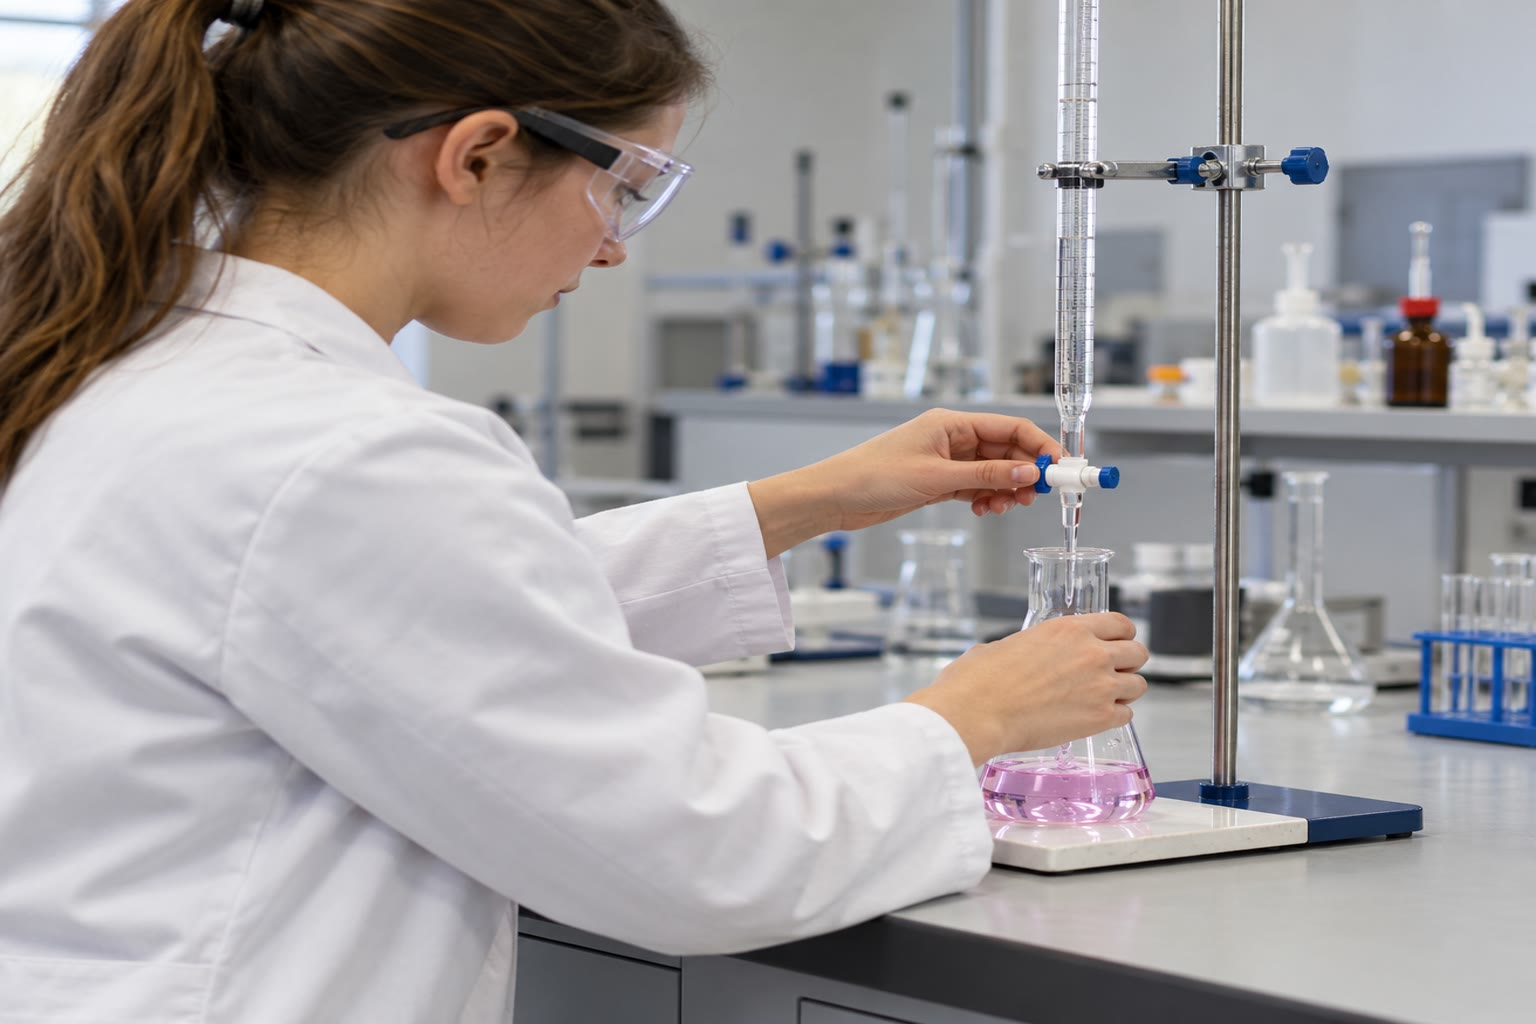
\includegraphics[width=0.48\linewidth]{images/book1/ai/g11-titration-bench.jpg}

{\small A \omterm{def:g11:titration:titration}{titration} in progress: burette, stand and conical flask on a
white tile.}
\end{omfigure}

\begin{remark}[How precise is a titration?]\label{rem:g11:titration:precision}
Each burette reading may be off by about \qty{0.05}{mL}, and the volume
poured is the difference of two readings: off by up to \qty{0.1}{mL}.
For $V_E = \qty{14.3}{mL}$, that is $0.1 / 14.3 \approx
\qty{0.7}{\percent}$. A larger $V_E$ makes this relative error smaller,
which is why \omterm{def:g11:titration:titration}{titrant} concentrations are chosen to give \omterm{def:g11:titration:equivalence}{equivalent
volumes} of 10 to \qty{20}{mL} with a \qty{25}{mL} burette. The
\omterm{def:g11:titration:titration}{titration} is repeated until two results agree within about
\qty{0.1}{mL}. A finer treatment of the uncertainty of a measurement is
given in the Year 1 volume.
\end{remark}

\begin{safety}{\ghs[0.7cm]{GHS03}\ghs[0.7cm]{GHS05}\ghs[0.7cm]{GHS07}\ghs[0.7cm]{GHS08}\ghs[0.7cm]{GHS09}}
% ledger: ghs:KMnO4, ghs:I2
Solid potassium permanganate is an \omterm{def:g11:redox:oxidant}{oxidant} that can feed a fire,
corrosive and harmful; its dilute solutions stain the skin and clothes
brown. Iodine solutions are harmful. Goggles and gloves; the waste is
collected, never poured down the sink.
\end{safety}

\section{Exercises}


\begin{exercise}[$\star$]\label{exo:g11:titration:1}
In a \omterm{def:g11:titration:titration}{titration}, what is the \omterm{def:g11:titration:titration}{titrant}? The \omterm{def:g11:titration:titration}{titrated solution}? What happens
at \omterm{def:g11:titration:equivalence}{equivalence}?
\end{exercise}

\begin{exercise}[$\star$]\label{exo:g11:titration:2}
What amount of permanganate \omterm{def:g9:ions:ion}{ions} is contained in \qty{12.5}{mL} of a
solution at \qty{0.0200}{mol/L}?
\end{exercise}

\begin{exercise}[$\star$]\label{exo:g11:titration:3}
On the figure of the amounts against the volume poured, read the
\omterm{def:g11:titration:equivalence}{equivalent volume}. What amount of iron(II) was in the flask at the
start?
\end{exercise}

\begin{exercise}[$\star$]\label{exo:g11:titration:4}
Why is no indicator needed for a \omterm{def:g11:titration:titration}{titration} by permanganate?
\end{exercise}

\begin{exercise}[$\star$]\label{exo:g11:titration:5}
At the \omterm{def:g11:titration:equivalence}{equivalence} of the \omterm{def:g11:titration:titration}{titration} of iron(II) by permanganate, what is
the ratio of the amount of iron(II) to the amount of permanganate
poured? Why?
\end{exercise}

\begin{exercise}[$\star\star$]\label{exo:g11:titration:6}
\qty{10.0}{mL} of an acidified iron(II) solution need \qty{8.40}{mL} of
permanganate at \qty{0.0200}{mol/L}. Compute the \omterm{def:g10:concentration-and-dilution:molar-concentration}{molar concentration} of
iron(II), then its \omterm{def:g10:concentration-and-dilution:mass-concentration}{mass concentration}.
\end{exercise}

\begin{exercise}[$\star\star$]\label{exo:g11:titration:7}
A vitamin C tablet is dissolved to make \qty{100.0}{mL} of solution.
\qty{10.0}{mL} of it, with starch, need \qty{11.4}{mL} of iodine at
\qty{0.0100}{mol/L}. What mass of vitamin C does the tablet contain?
\end{exercise}

\begin{exercise}[$\star\star$]\label{exo:g11:titration:8}
A reaction is total but takes several minutes. Why can it not be used as
it is for a \omterm{def:g11:titration:titration}{titration} with a colour change?
\end{exercise}

\begin{exercise}[$\star\star$]\label{exo:g11:titration:9}
Look at the three flasks. A student stops at a flask as purple as the
third one. Is her \omterm{def:g11:titration:equivalence}{equivalent volume} too large or too small? What should
she have done near \omterm{def:g11:titration:equivalence}{equivalence}?
\end{exercise}

\begin{exercise}[$\star\star$]\label{exo:g11:titration:10}
A concentrated iron(II) solution is first diluted ten times. Then
\qty{10.0}{mL} of the diluted solution need \qty{13.0}{mL} of
permanganate at \qty{0.0200}{mol/L}. Find the concentration of the
concentrated solution.
\end{exercise}

\begin{exercise}[$\star\star$]\label{exo:g11:titration:11}
% ledger: aw:Fe
The iron(II) solution of the chapter's worked example has
$c = \qty{0.0630}{mol/L}$. What mass of iron does \qty{1.00}{L} of it
contain?
\end{exercise}

\begin{exercise}[$\star\star\star$]\label{exo:g11:titration:12}
A \omterm{def:g11:titration:titration}{titration} gives $V_E = \qty{7.2}{mL}$. Estimate the relative error due
to the burette readings, and compare with $V_E = \qty{14.3}{mL}$. Suggest
two ways of obtaining a larger \omterm{def:g11:titration:equivalence}{equivalent volume}.
\end{exercise}

\begin{exercise}[$\star\star\star$]\label{exo:g11:titration:13}
Hydrogen peroxide is titrated by permanganate in acid:
\[
  \ce{2MnO4^- + 5H2O2 + 6H+ -> 2Mn^{2+} + 5O2 + 8H2O} .
\]
A disinfectant is diluted ten times; \qty{10.0}{mL} of the diluted
solution need \qty{17.6}{mL} of permanganate at \qty{0.0200}{mol/L}.
Find the \omterm{def:g10:concentration-and-dilution:molar-concentration}{molar concentration} of hydrogen peroxide in the disinfectant,
then its \omterm{def:g10:concentration-and-dilution:mass-concentration}{mass concentration} (\ce{H2O2}: \qty{34.0}{g/mol}).
\end{exercise}

\begin{exercise}[$\star\star\star$]\label{exo:g11:titration:14}
An iron tablet should contain about \qty{1.4e-3}{mol} of iron(II). What
concentration of permanganate gives an \omterm{def:g11:titration:equivalence}{equivalent volume} near
\qty{15}{mL} with a \qty{25}{mL} burette? What would go wrong with a
solution ten times more concentrated?
\end{exercise}

\begin{exercise}[$\star\star\star$]\label{exo:g11:titration:15}
The equation of the \omterm{def:g11:titration:titration}{titration} shows \ce{8H+} for each \ce{MnO4^-}. For an
\omterm{def:g11:titration:equivalence}{equivalent volume} of \qty{14.3}{mL} at \qty{0.0200}{mol/L}, what amount of
hydrogen \omterm{def:g9:ions:ion}{ions} is used up? Is \qty{10}{mL} of an acid containing
\qty{1.0}{mol/L} of hydrogen \omterm{def:g9:ions:ion}{ions} enough? Why must the flask be
acidified?
\end{exercise}

\section{Problem: Is the Iron Tablet Honest?}

\begin{problem}[{Weekend problem --- an iron supplement claims 80 mg of
iron per tablet: does a titration agree?}]
\label{pb:g11:titration:1}
% ledger: aw:Fe, aw:S, aw:O, const:NA
The box of an iron supplement claims \qty{80}{mg} of iron, as iron(II),
per tablet. A tablet is crushed and dissolved in about \qty{50}{mL} of
dilute sulfuric acid, then titrated by potassium permanganate at
\qty{0.0200}{mol/L}. The faint pink persists at $V_E = \qty{14.3}{mL}$.

\medskip
\noindent\textbf{Part I --- The reaction.}
\begin{enumerate}
  \item Name the two \omterm{def:g11:redox:couple}{redox couples} involved. Which species is the
        \omterm{def:g11:redox:oxidant}{oxidant}, which the \omterm{def:g11:redox:oxidant}{reductant}?
  \item Write the two \omterm{def:g11:redox:couple}{half-equations}.
  \item Combine them into the equation of the \omterm{def:g11:titration:titration}{titration}, and check that
        it is balanced in charge.
  \item Why is the tablet dissolved in acid?
  \item Show that the reaction meets the conditions of a \omterm{def:g11:titration:titration}{titration}, and
        explain how \omterm{def:g11:titration:equivalence}{equivalence} is seen.
\end{enumerate}

\medskip
\noindent\textbf{Part II --- The \omterm{def:g11:titration:titration}{titration}.}
\begin{enumerate}[resume]
  \item In which piece of glassware is the permanganate solution? How is
        its volume read?
  \item What colour is the flask before \omterm{def:g11:titration:equivalence}{equivalence}, and why does each
        drop lose its colour?
  \item Compute the amount of permanganate poured at \omterm{def:g11:titration:equivalence}{equivalence}.
\end{enumerate}

\medskip
\noindent\textbf{Part III --- The iron.}
\begin{enumerate}[resume]
  \item Deduce the amount of iron(II) in the tablet.
  \item Compute its mass in milligrams.
  \item Compare with the label: relative difference?
  \item The volume poured may be off by \qty{0.1}{mL}. By how many
        milligrams may the mass of iron be off? Is the label confirmed?
\end{enumerate}

\medskip
\noindent\textbf{Part IV --- Several tablets.}
\begin{enumerate}[resume]
  \item Two more tablets give $V_E = \qty{14.1}{mL}$ and
        \qty{14.4}{mL}. Compute their masses of iron.
  \item Compute the mean of the three tablets.
  \item The three results differ by more than the burette error. What
        does this say about the tablets?
  \item Would permanganate at \qty{0.100}{mol/L} have been a better
        choice? Explain.
  \item Many supplements also contain vitamin C, a \omterm{def:g11:redox:oxidant}{reductant}. What would
        it do to the \omterm{def:g11:titration:titration}{titration}, and to the mass of iron found?
  \item The iron is present as iron(II) sulfate, \ce{FeSO4}. What mass of
        it does one tablet contain?
  \item How many iron(II) \omterm{def:g9:ions:ion}{ions} is that?
  \item State the final answer: what mass of iron does one tablet
        contain?
\end{enumerate}
\end{problem}
